\subsection{Ejercicio 5}
\graphicspath{ {img/05} }

\subsubsection{Proceso para obtener certificado digital FNMT}

Lo primero que se debe hacer para obtener el certificado digital es entrar en la web de la Fábrica Nacional de Moneda y Timbre (FNMT). Una vez ahí, seleccionamos la opción “Obtener certificado digital como persona física”. Se verá en la pantalla la \ref{fig:web_ej5a}. 

\begin{figure}[H]   
    \centering
    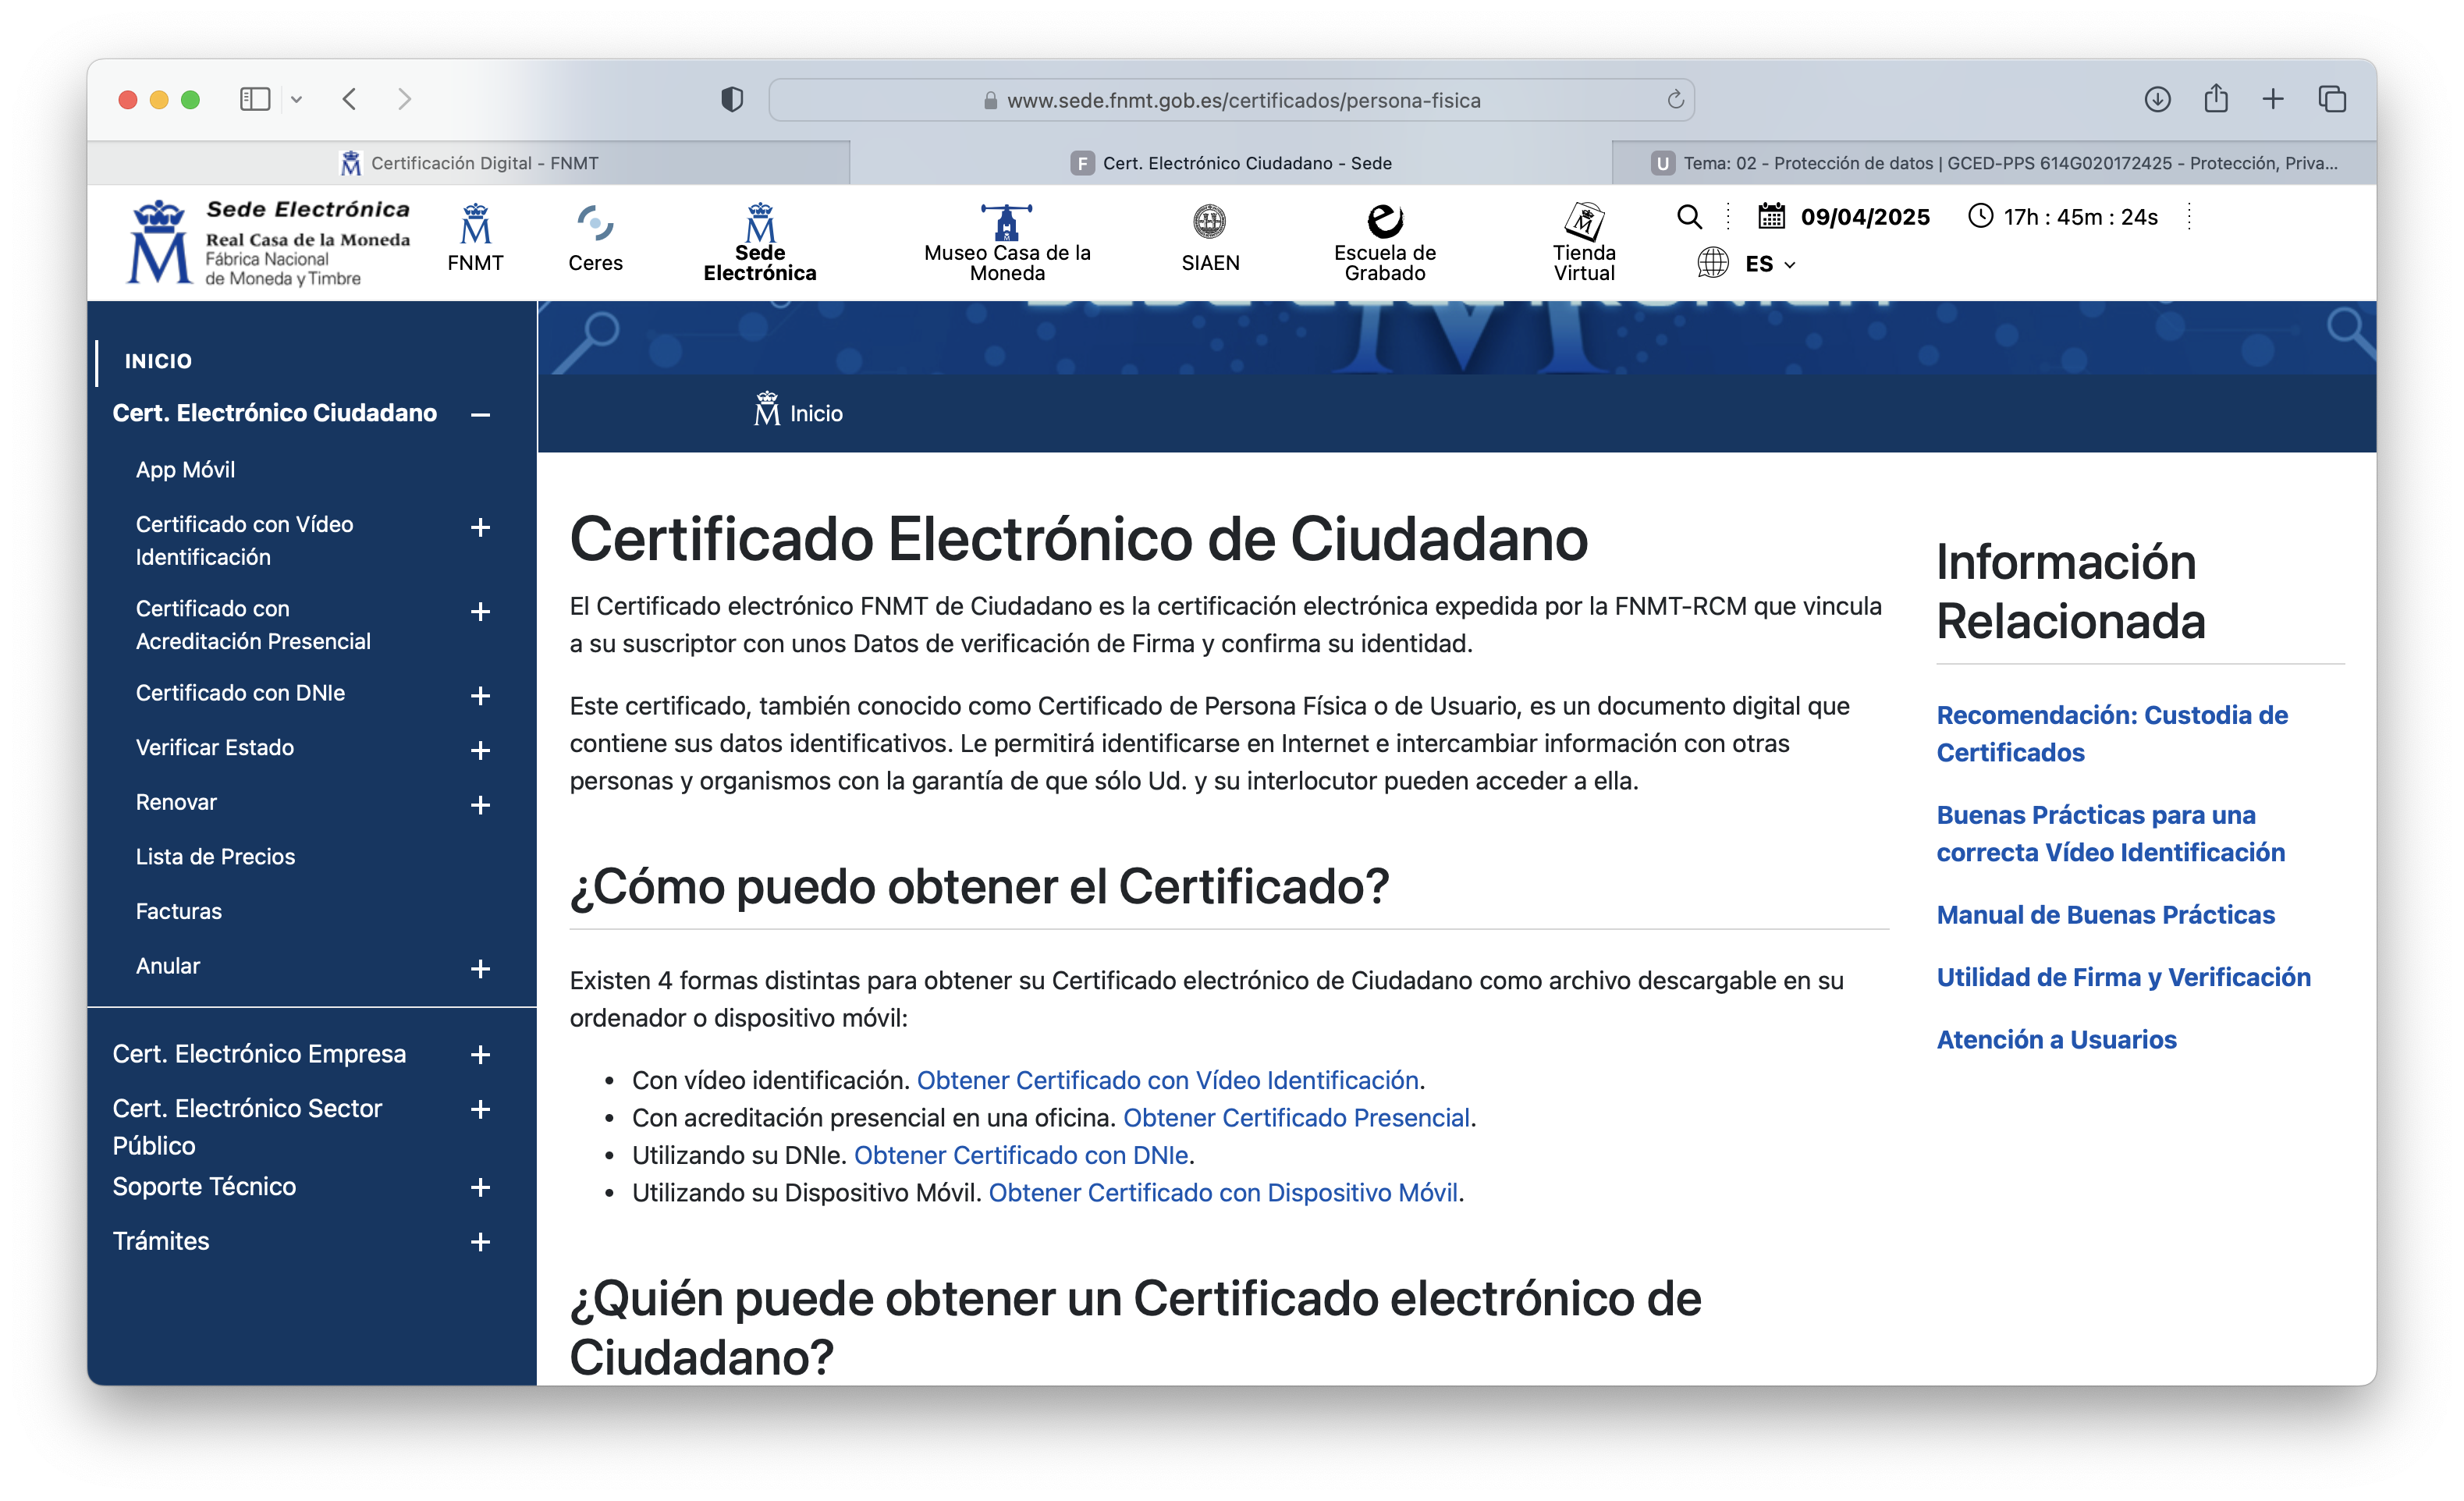
\includegraphics[width=\textwidth]{web_ej5a.png}
    \caption{Página inicio web FNMT}
    \label{fig:web_ej5a}
\end{figure}

En ella se ven las 4 formas a través de las que podemos conseguir el certificado. En nuestro caso, se eligió la opción de "Obtener certificado presencial". Una vez seleccionada la opción, como se ve en la \ref{fig:paso1}, se nos explican 4 pasos a seguir para obtener nuestro certificado. 

El paso 1 consiste en una configuración previa. Se debe instalar una aplicación para solicitar las claves necesarias en la obtención de un certificado digital. Puede ser ejecutada en cualquier navegador y sistema Operativo. Una vez descargado e instalado el software no es necesario hacer nada, este se ejecutará cuando el navegador lo requiera. En la \ref{fig:instalacion_FNMT}, se ve el final de la instalación del software. En la propia instalación se crea la contraseña, necesaria para el paso final. 

\begin{figure}[H]   
    \centering
    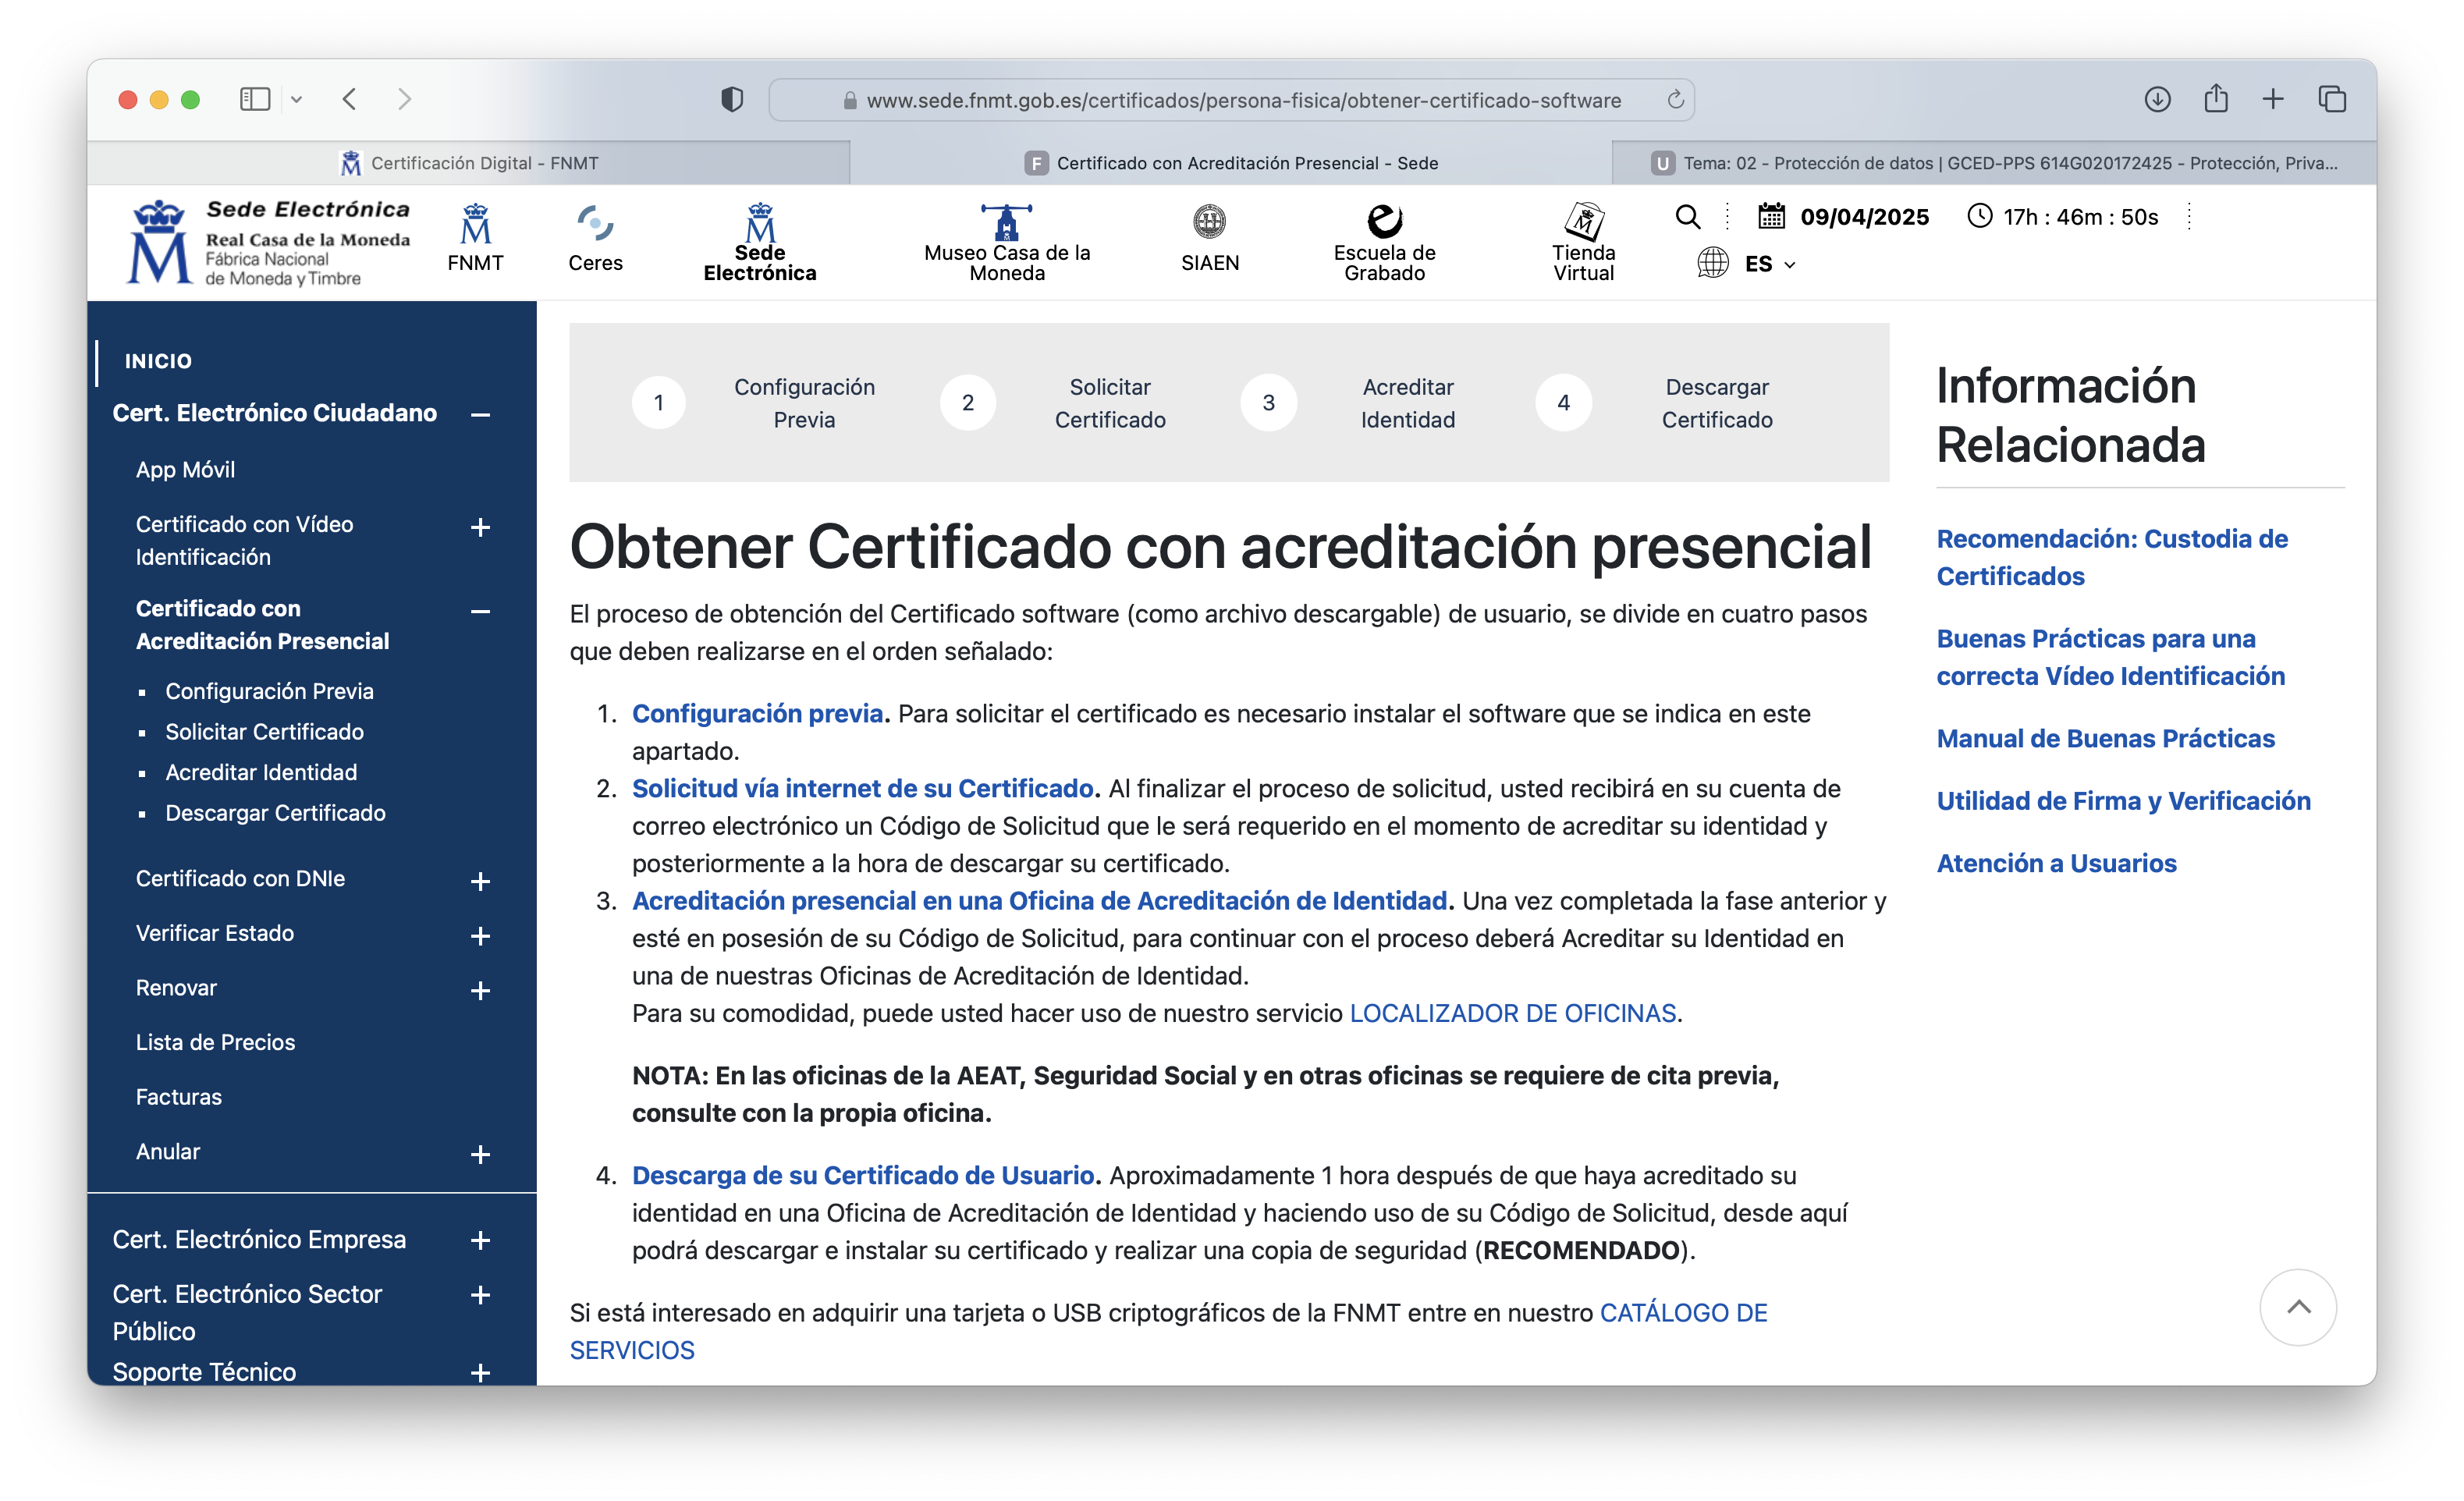
\includegraphics[width=\textwidth]{paso1_ej5a.png}
    \caption{Paso 1}
    \label{fig:paso1}
\end{figure}

\begin{figure}[H]   
    \centering
    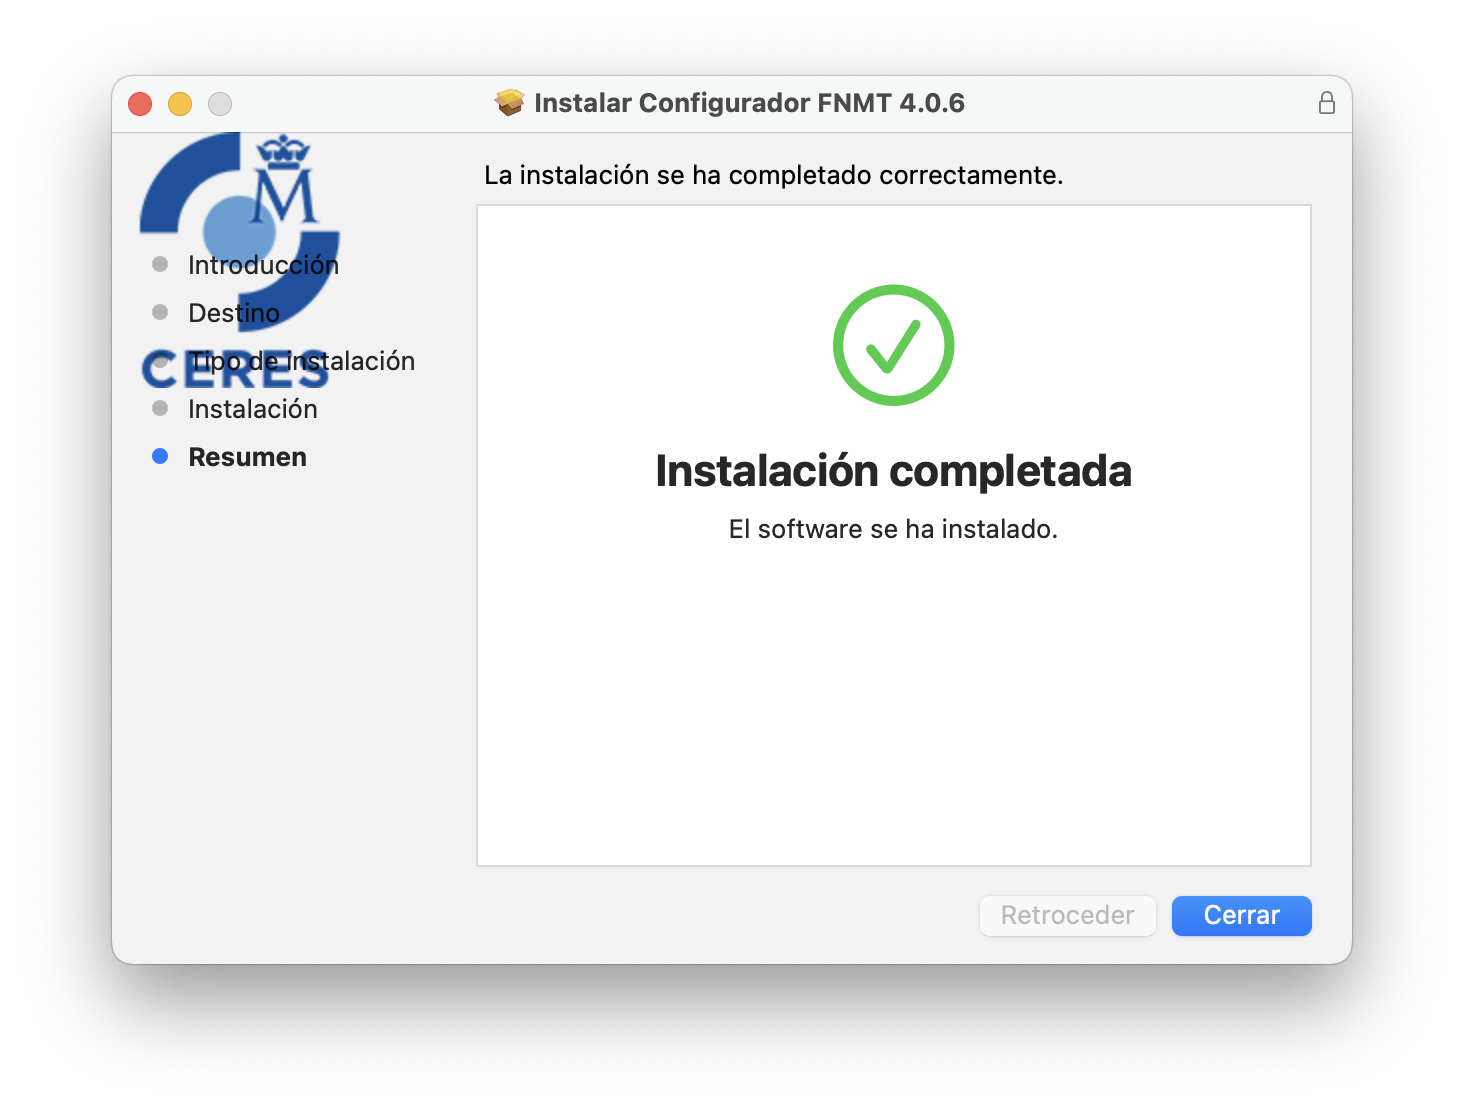
\includegraphics[width=\textwidth]{instalacion_FNMT_ej5a.png}
    \caption{Instalación software FNMT}
    \label{fig:instalacion_FNMT}
\end{figure}

Una vez instalado el software, proseguimos con el paso 2. En este paso debemos cubrir un formulario para solicitar el certificado. En la \ref{fig:paso2} se ve el formulario a cubrir. Tras la solicitud, se recibe un correo electrónico que incluye un código de solicitud. 

\begin{figure}[H]   
    \centering
    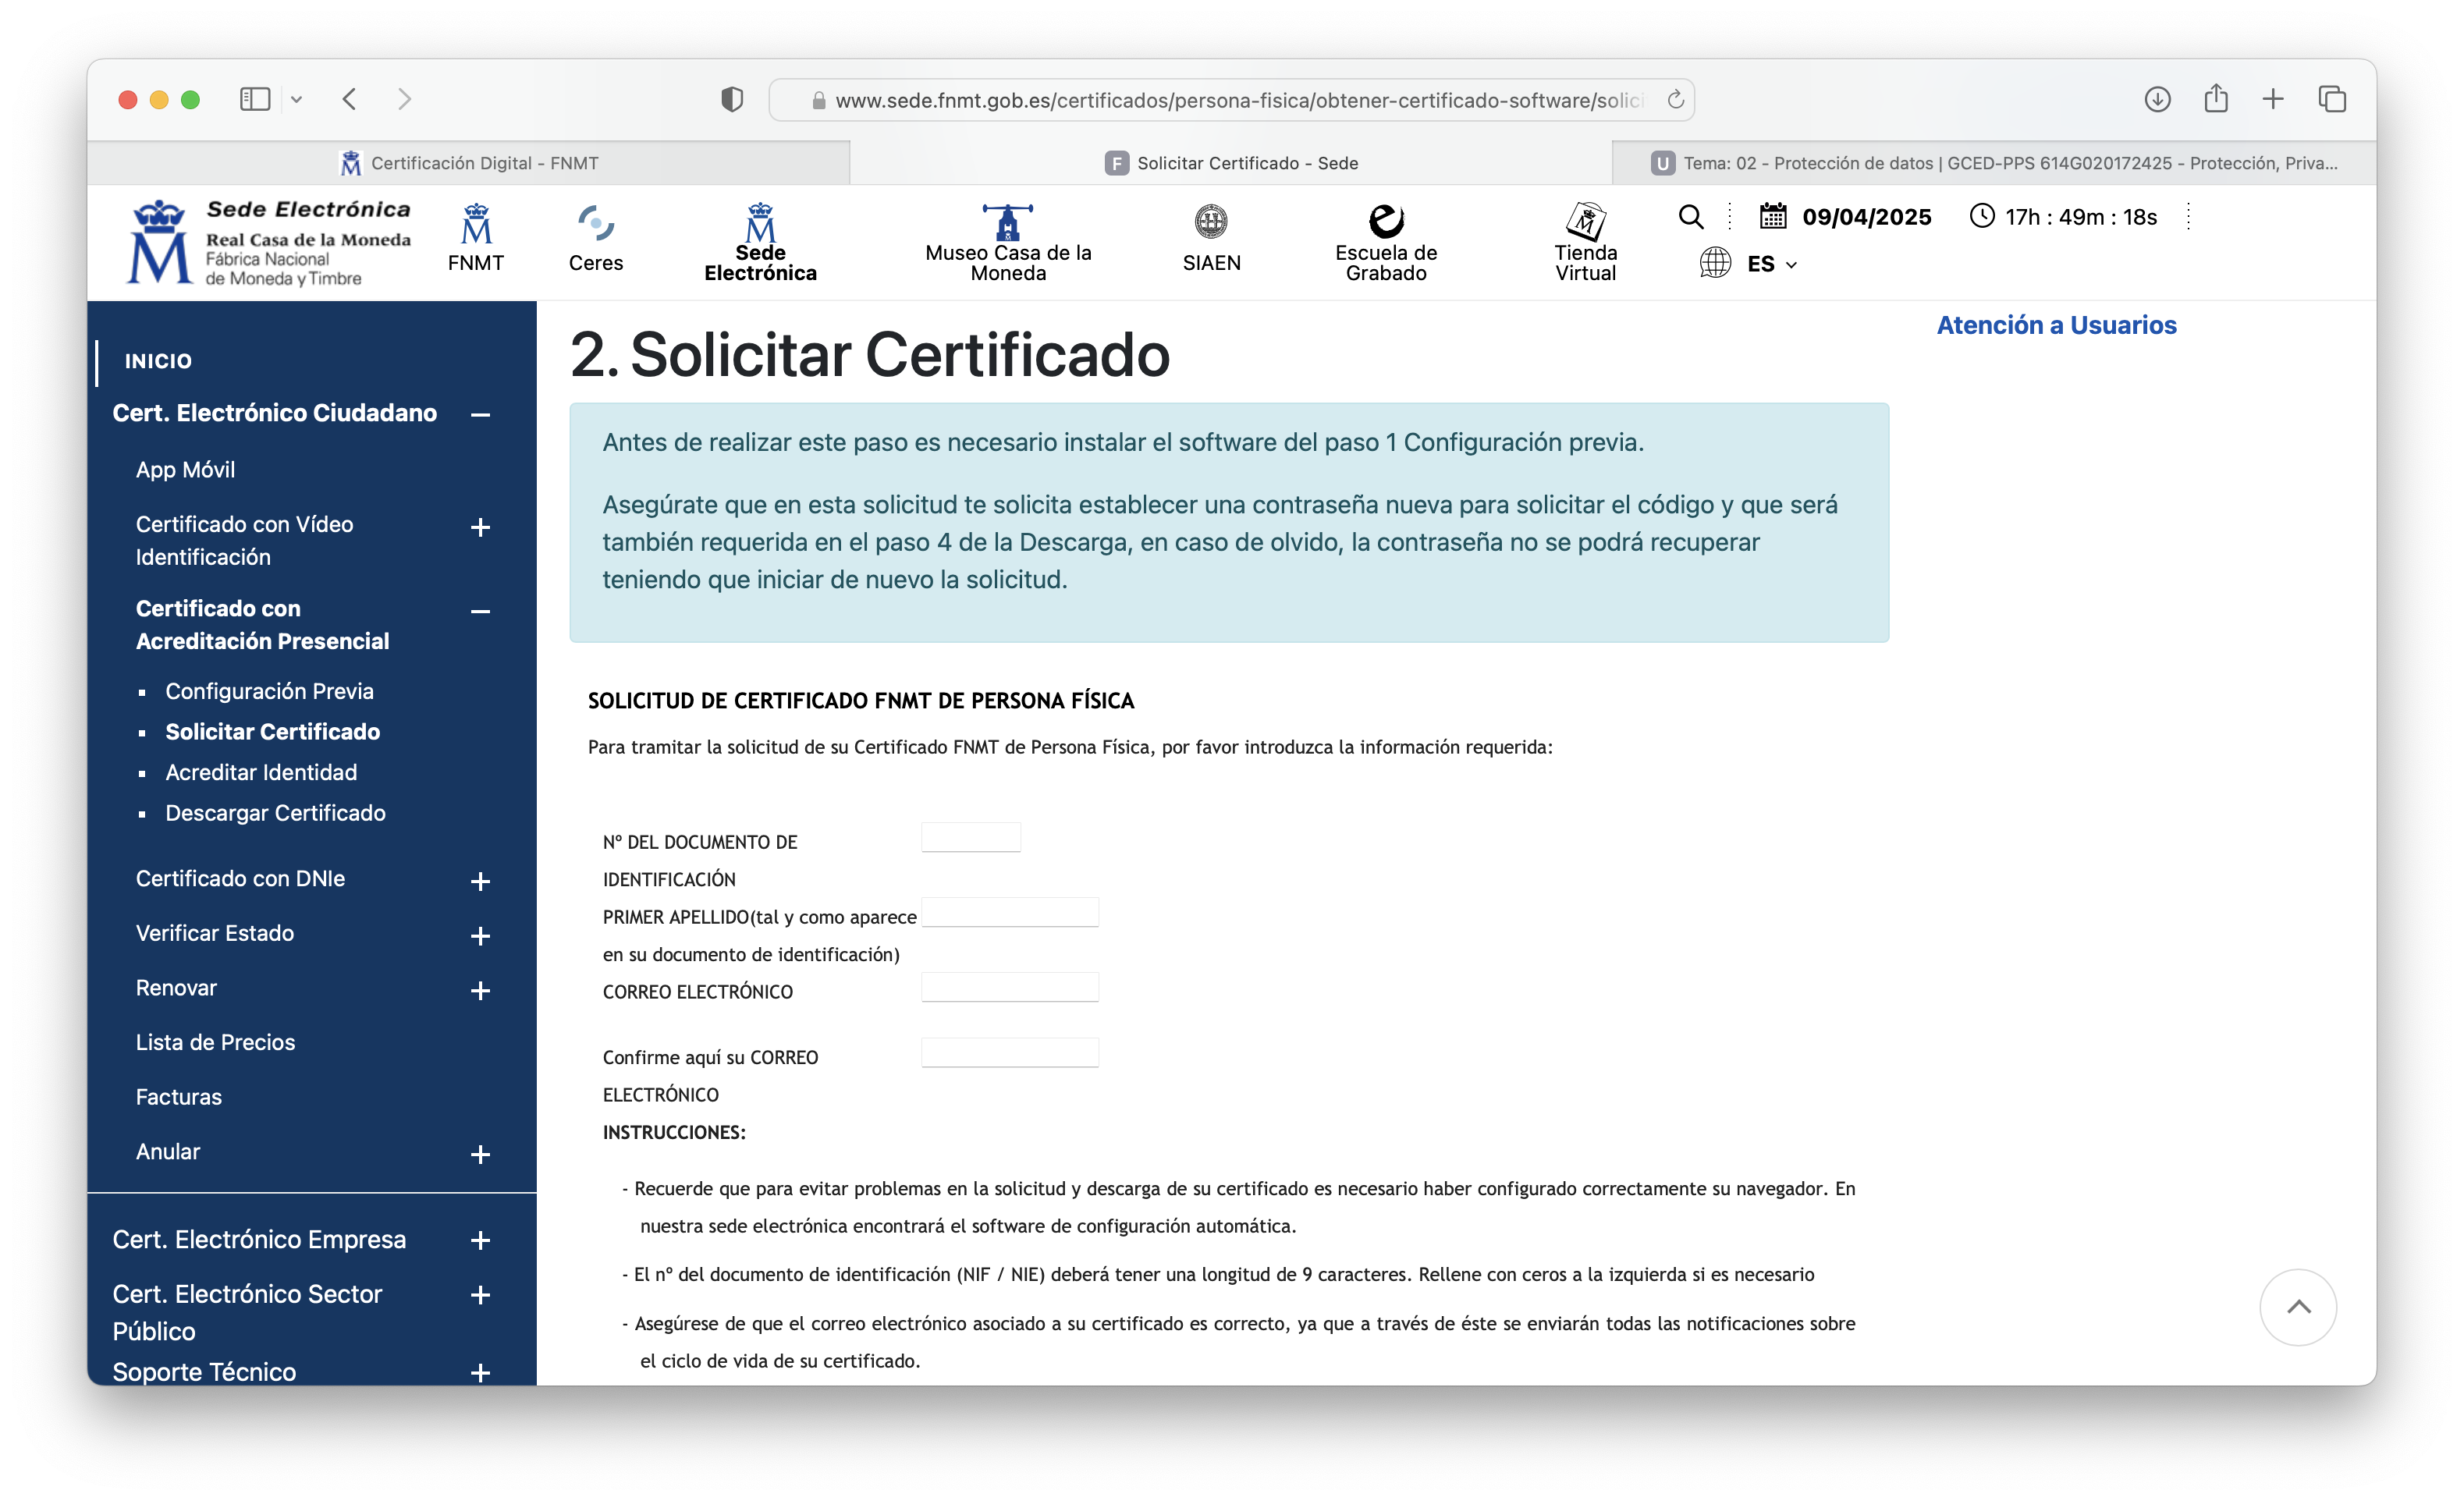
\includegraphics[width=\textwidth]{paso2_ej5a.png}
    \caption{Paso 2}
    \label{fig:paso2}
\end{figure}

El tercer paso consiste en acudir presencialmente a una oficina de registro habilitada con nuestro DNI físico y el código de solicitud obtenido en el correo electrónico del paso anterior. Allí, nos identificaron presencialmente y validaron nuestra identidad. En la página web de la FNMT se puede encontrar el mapa de la \ref{fig:mapa}, con las oficinas a las que podemos acudir, en nuestro caso, hacienda. Tras la cita, recibiremos otro correo electrónico. 

\begin{figure}[H]   
    \centering
    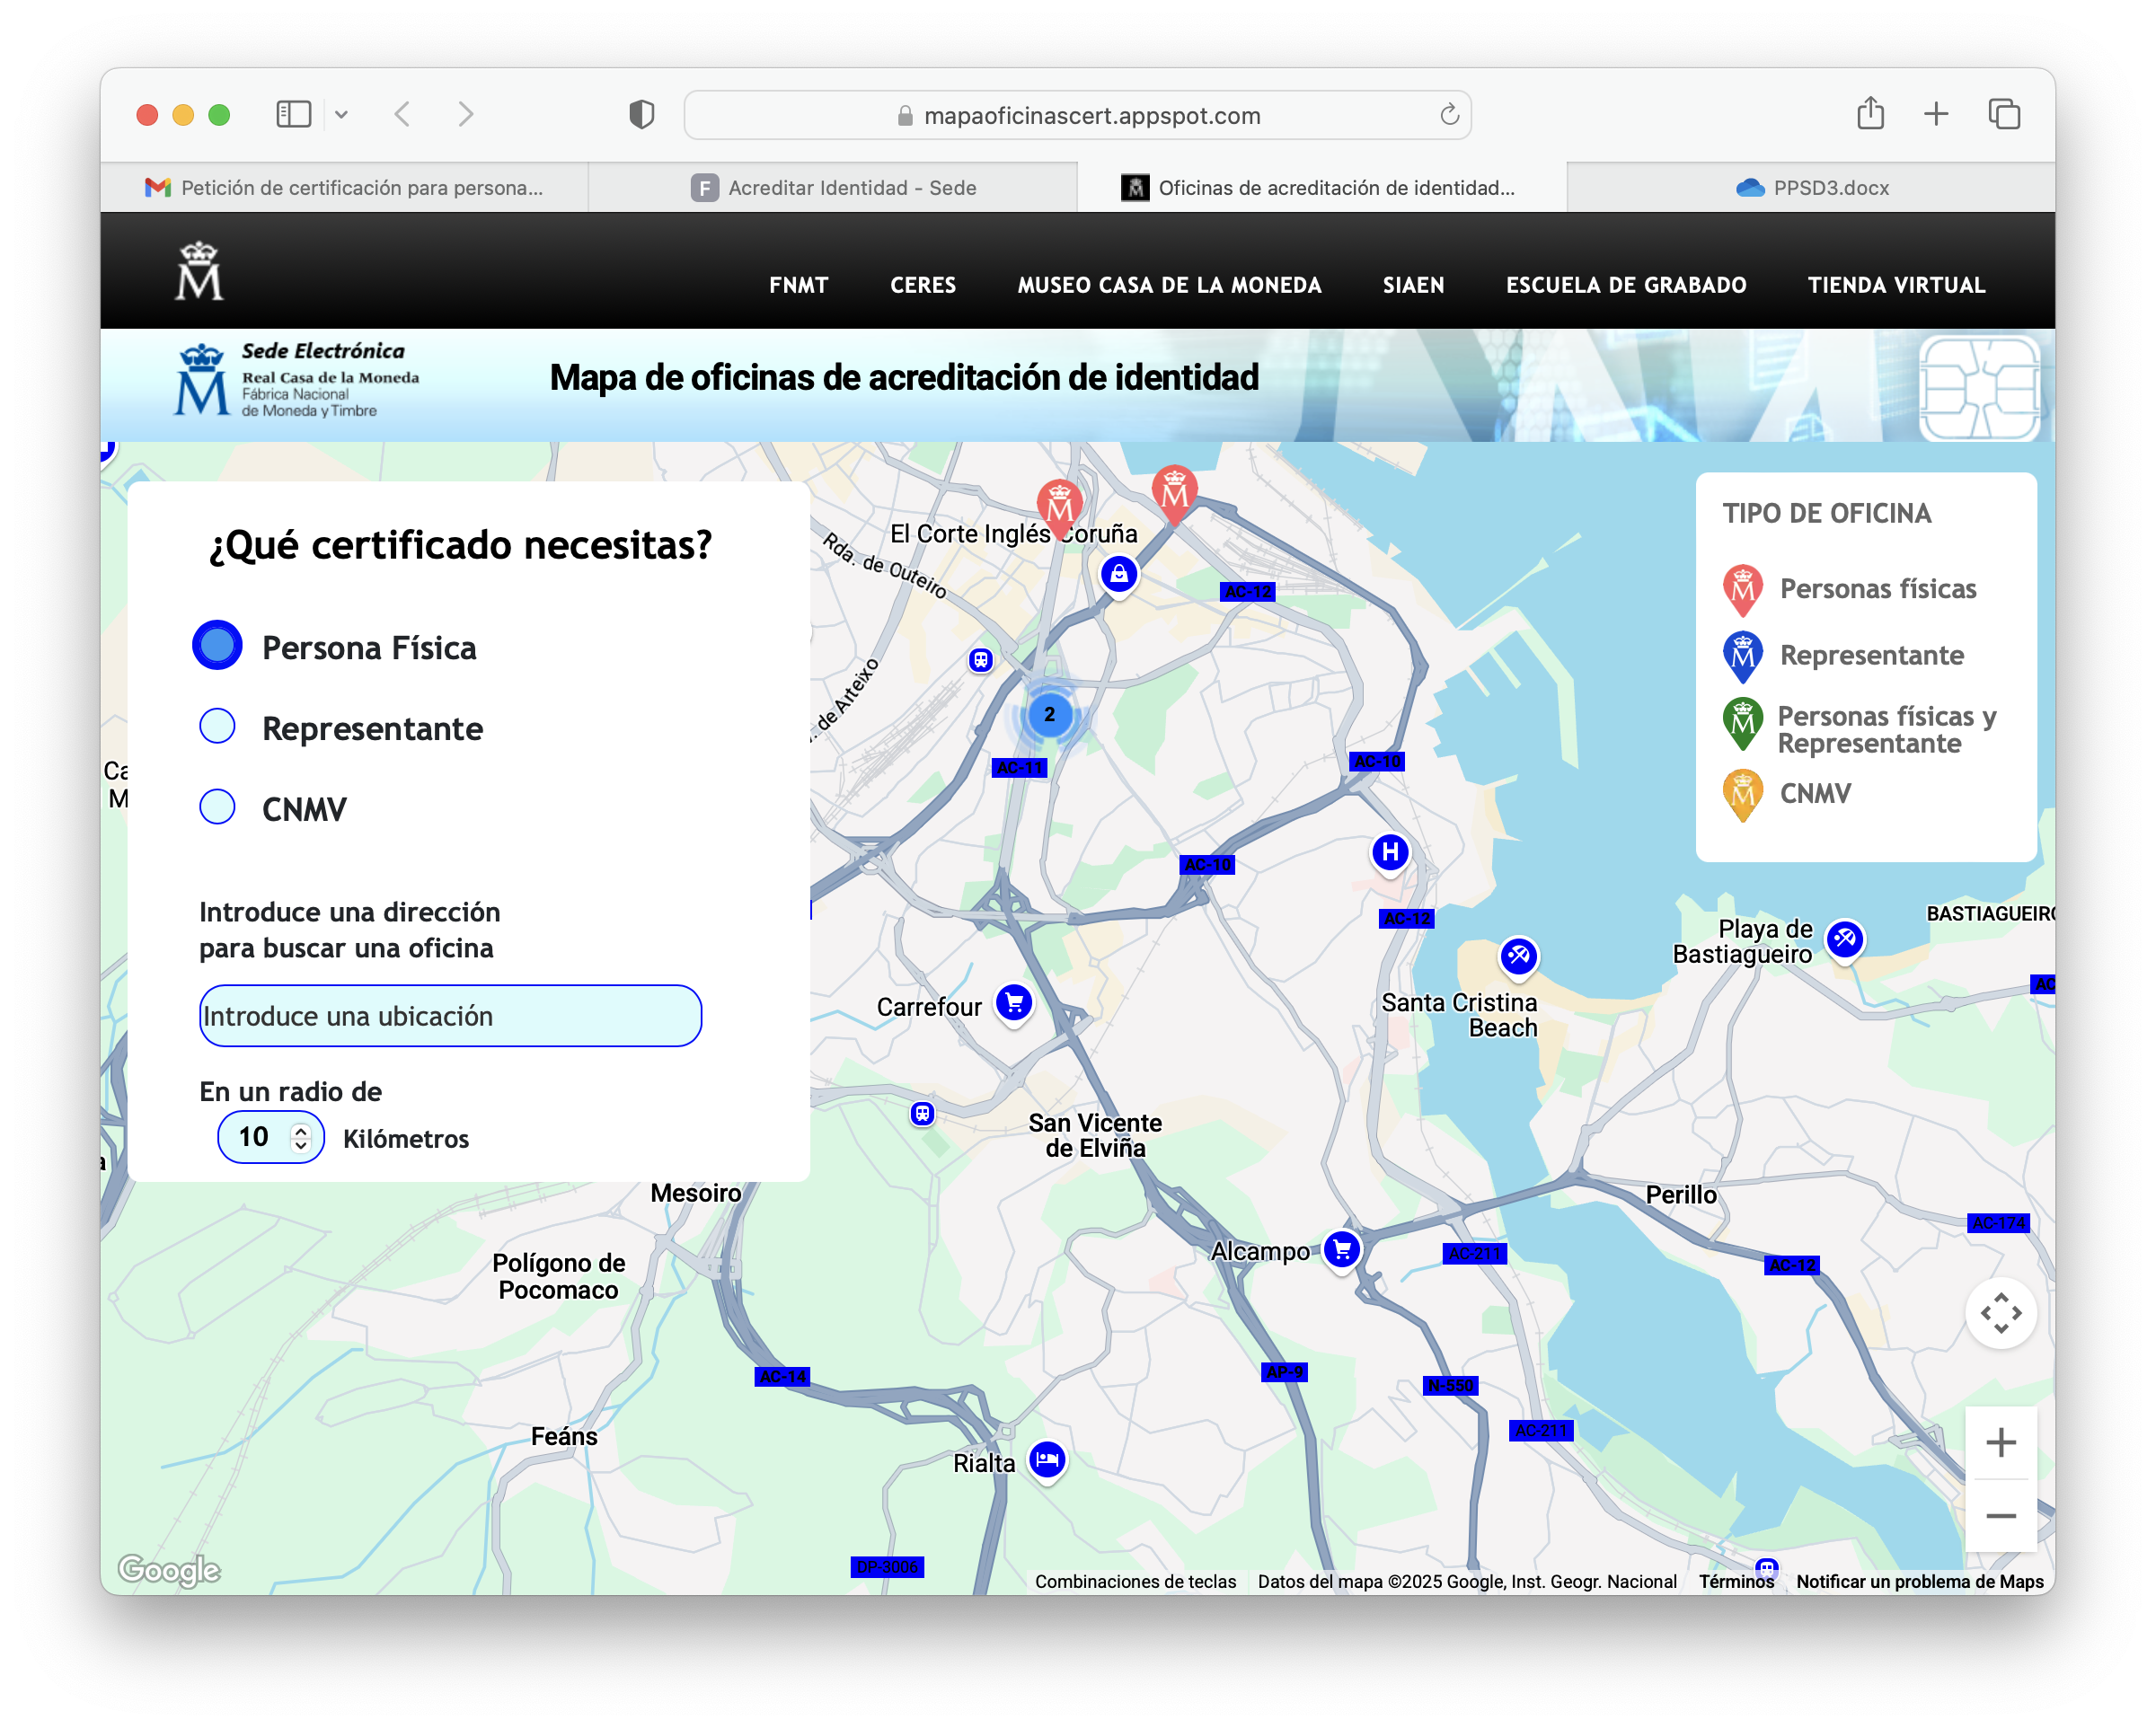
\includegraphics[width=\textwidth]{mapa_ej5a.png}
    \caption{Mapa oficinas de acreditación}
    \label{fig:mapa}
\end{figure}

El último paso consiste en descargar el certificado en el mismo navegador y equipo con el que se hizo la solicitud. En el correo electrónico recibido tras acudir a hacienda, se nos proporciona la confirmación de nuestra solicitud, así como el enlace al formulario de la \ref{fig:paso4}. Una vez cubierto, el navegador instala el certificado, vinculando la clave privada local con el certificado emitido por la FNMT. Se debe ver un mensaje como el de la \ref{fig:fin_instalacion}. Es recomendable descargar el certificado en nuestro dispositivo.  

\begin{figure}[H]   
    \centering
    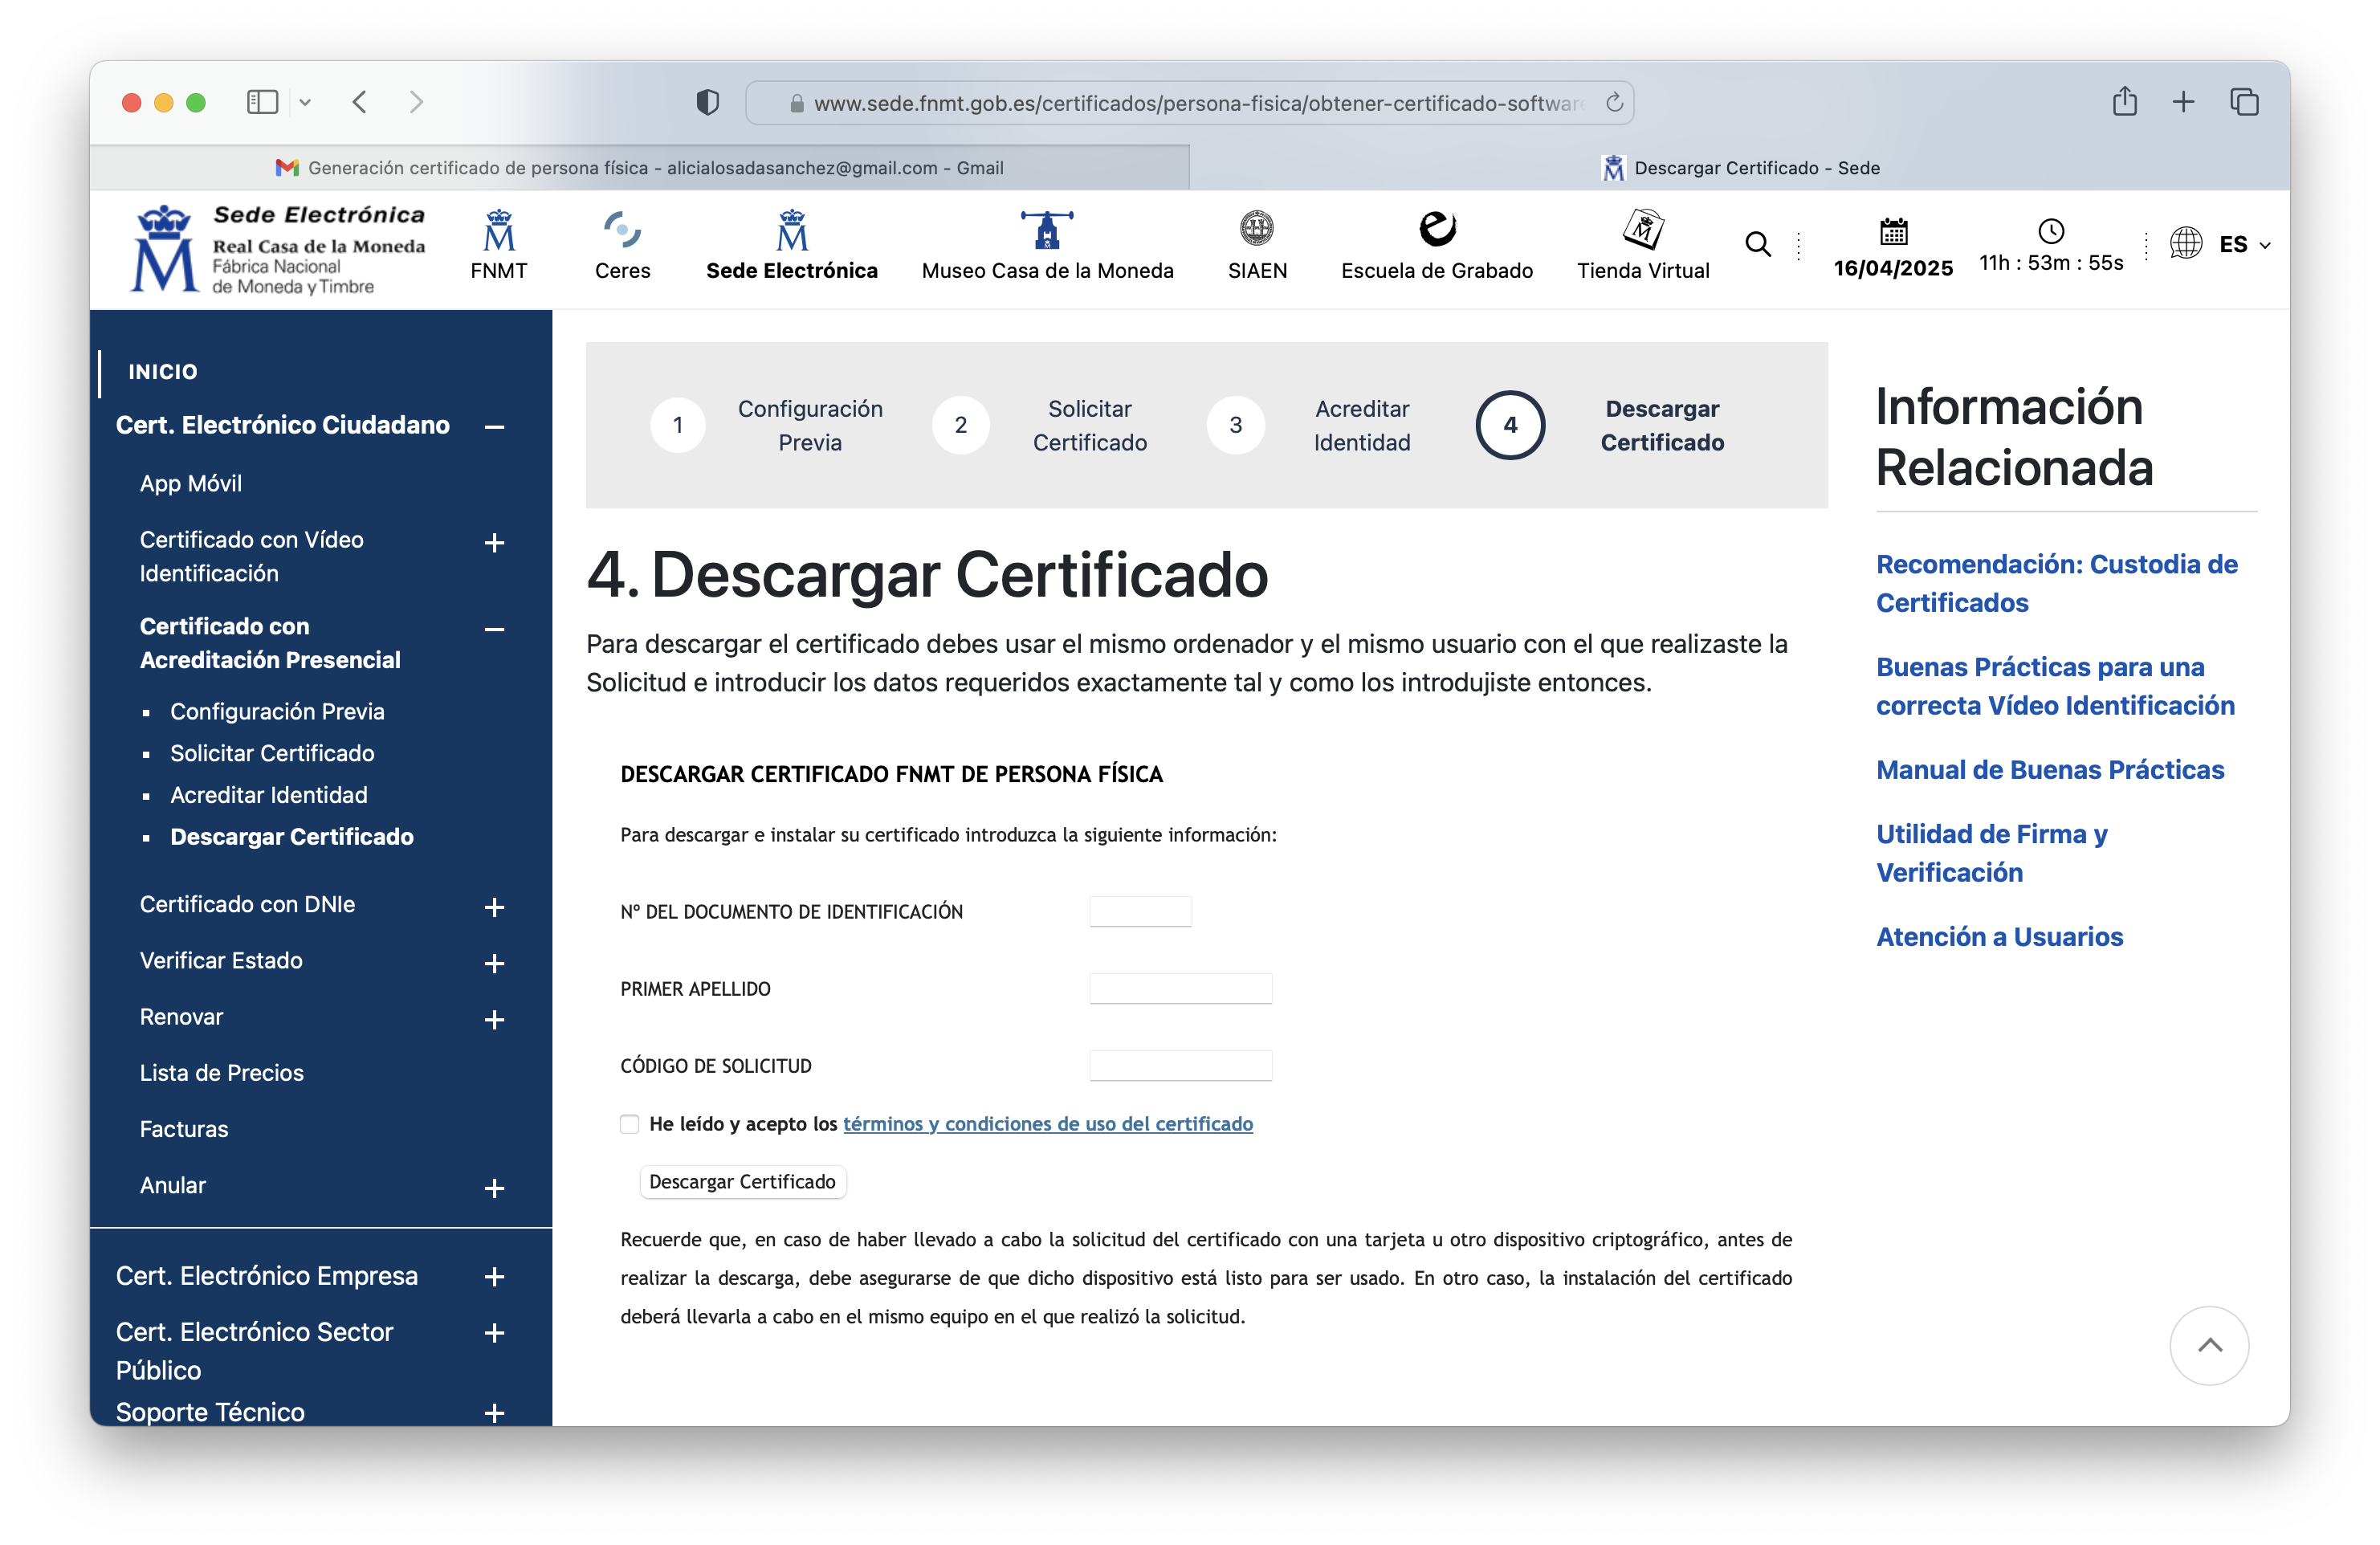
\includegraphics[width=\textwidth]{paso4_ej5a.png}
    \caption{Paso 4}
    \label{fig:paso4}
\end{figure}

\begin{figure}[H]   
    \centering
    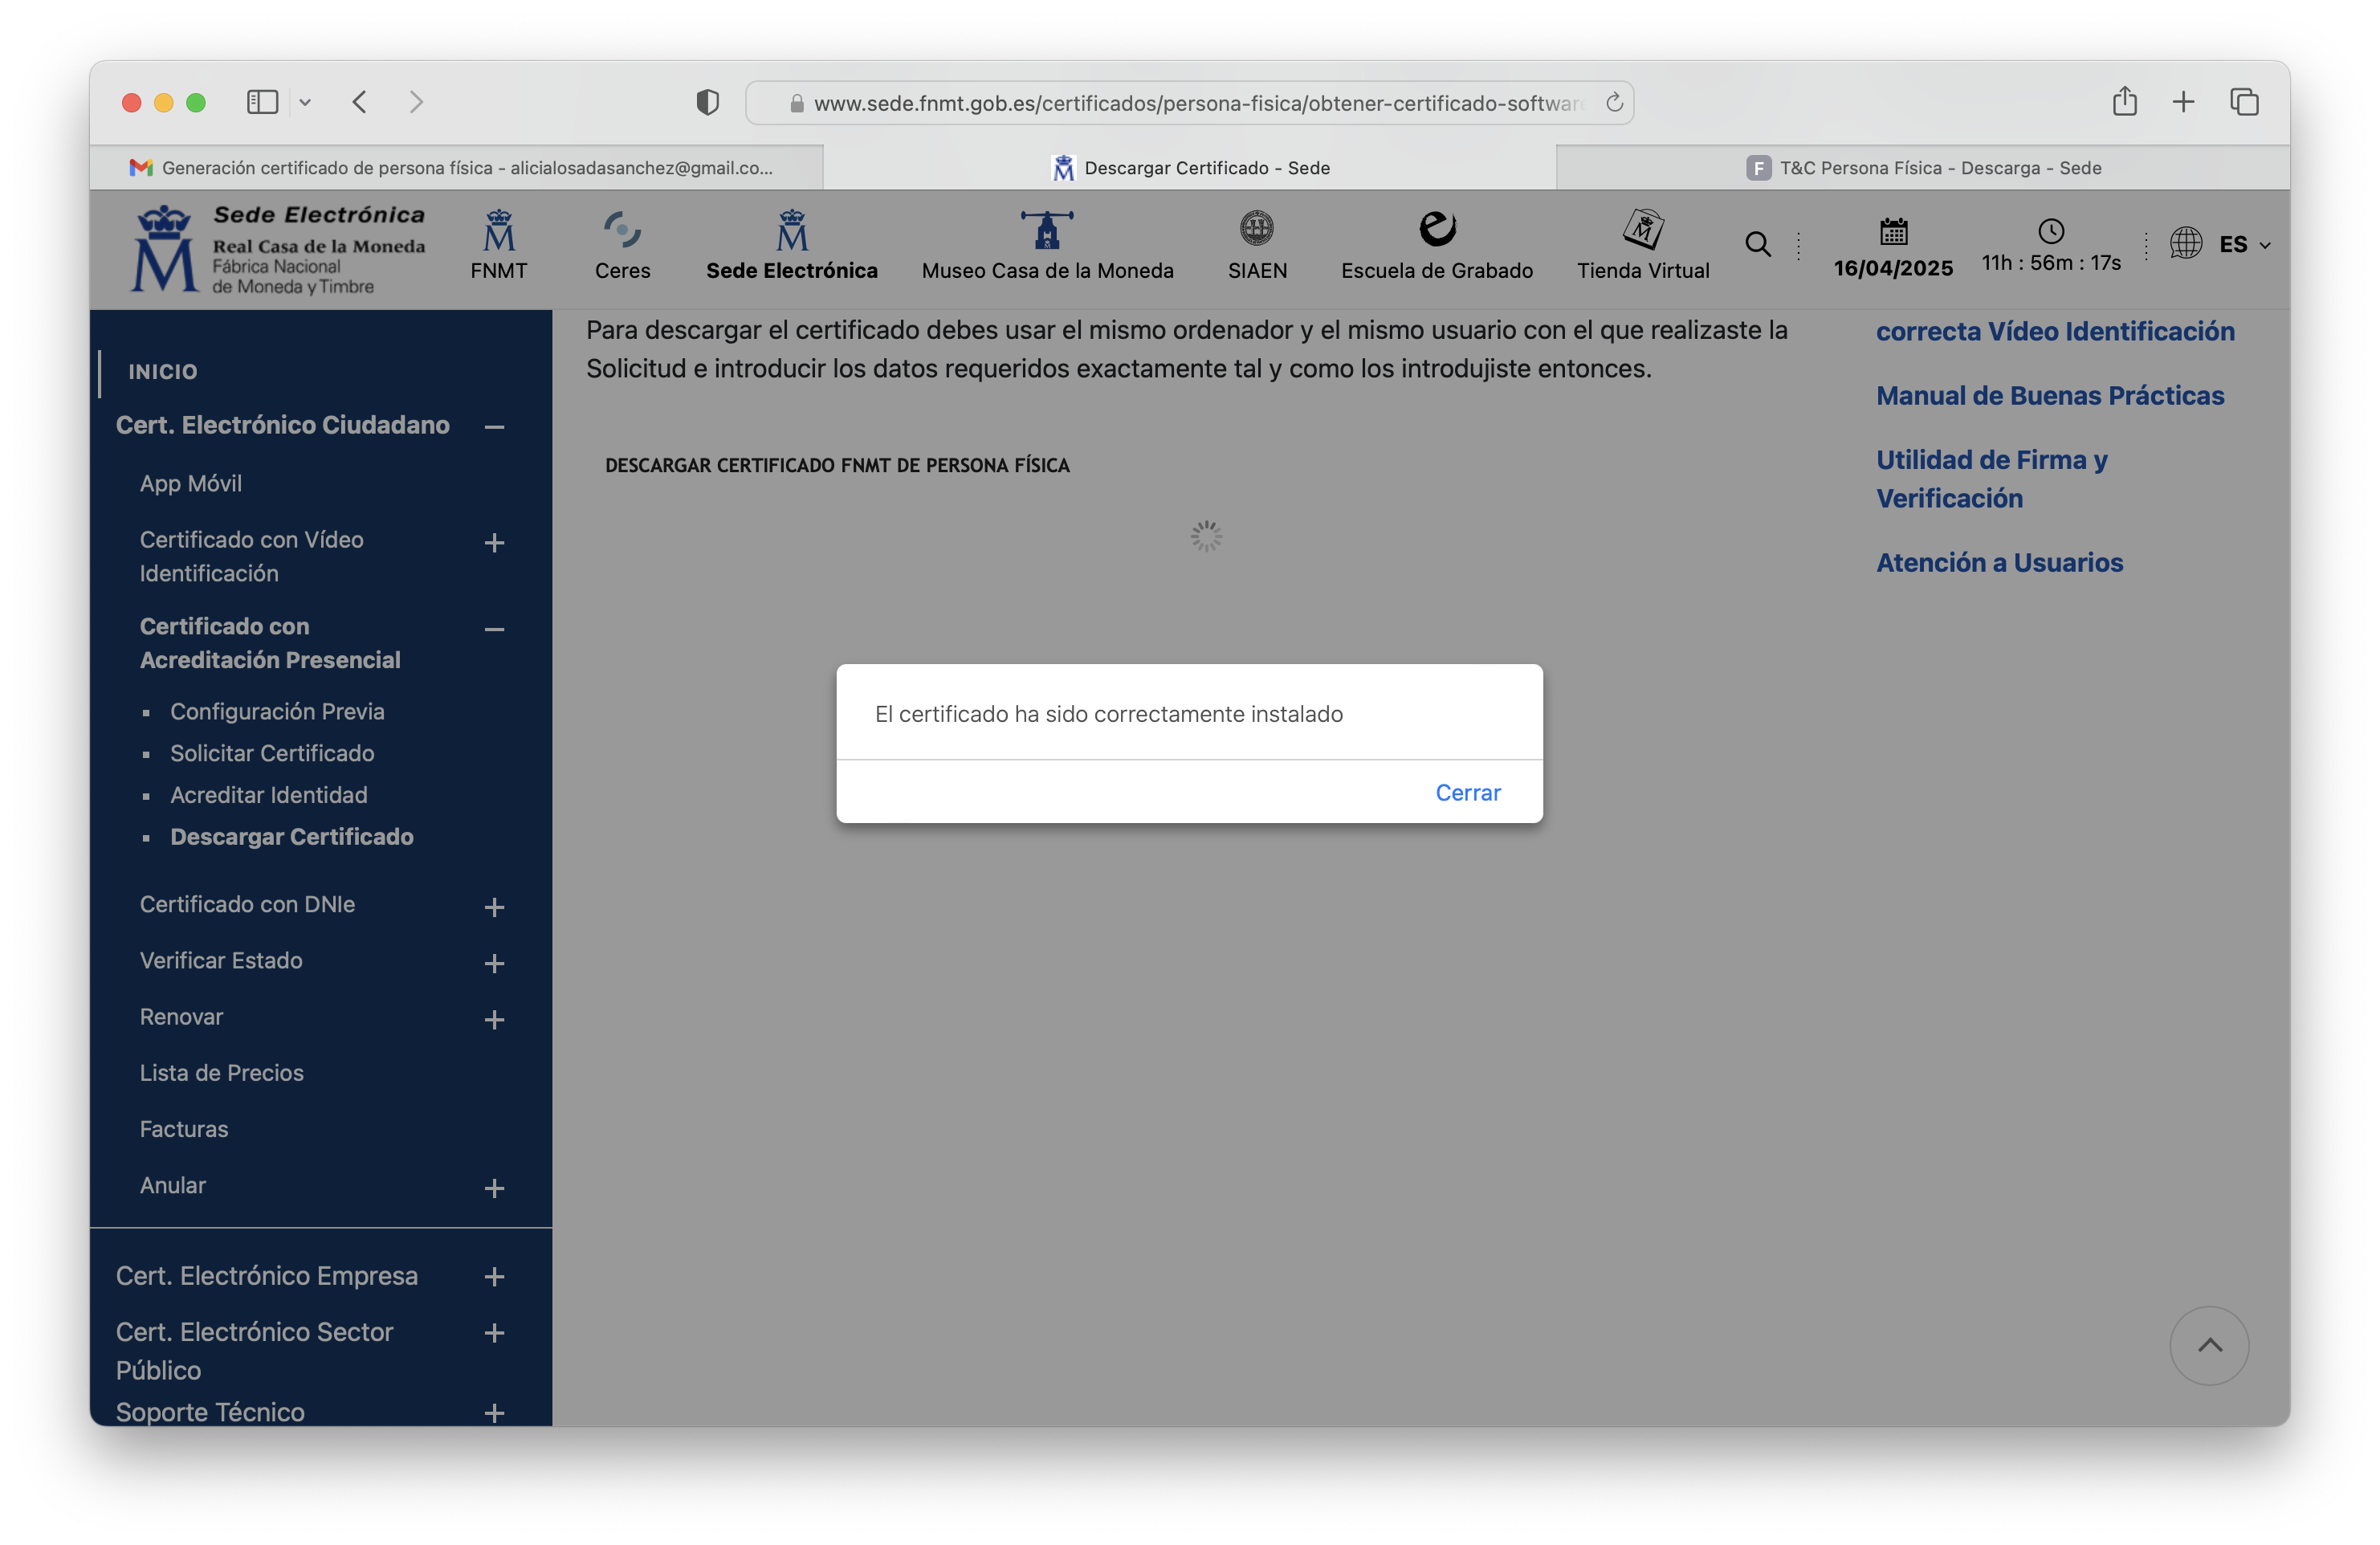
\includegraphics[width=\textwidth]{fin_instalacion_ej5a.png}
    \caption{Fin instalación certificado}
    \label{fig:fin_instalacion}
\end{figure}

Las claves se generan en el propio navegador del usuario en el momento en que se realiza la solicitud del certificado digital en la web de la FNMT. Específicamente, el navegador crea un par de claves: una clave pública, que se envía a la Autoridad Certificadora (CA), y una clave privada, que nunca abandona el equipo del usuario.  

Esta clave privada se almacena localmente en el almacén de certificados del navegador o del sistema operativo, dependiendo del navegador utilizado. Por ejemplo, en Firefox se guarda en su propio almacén interno, mientras que en navegadores como Chrome o Edge en Windows, se almacena en el almacén de certificados del sistema operativo. 


\subsubsection{Análisis campos clave pública OpenSSL}

